%%%%%%%%%%%%%%%%%%%%%%% CHAPTER - 6 %%%%%%%%%%%%%%%%%%%%\\
\chapter{Large Vocabulary Pronunciation Lexicons for Malayalam ASR} \label{ch:lvcsr} %%%%%%%%%%%%%%%%%%%%%%%%%%%%

\graphicspath{{Figures/chapter5-lvcsr}}

\section{Introduction}

This chapter discusses the development of an \gls{lvcsr} system for Malayalam using the pipeline approach, which includes building a large vocabulary pronunciation lexicon. A comprehensive and robust \gls{pl} should be able to handle the language's complex phonology. To achieve this, we utilise an automated approach using Mlphon, an \gls{fst}-based toolkit developed as part of this research and described in detail in Chapter \ref{ch:Mlphon}.

Using Mlphon we publish a large vocabulary pronunciation lexicon for Malayalam in both phonemized and syllabified forms. It contains more than 100,000 words covering different categories of words. It is the first of its kind resource available in Malayalam language. To evaluate the effectiveness of the \gls{pl} created using Mlphon, we compare it with those created using other automated tools such as Unified Parser and Espeak. We perform a qualitative comparative analysis of the \gls{pl} generated by different tools, while also evaluating the word processing speed of each. 

To build the Malayalam \gls{lvcsr} model, we combine the lexicons generated using automated tools with a statistical \gls{lm} and a hybrid \gls{dnn}-\gls{hmm} acoustic model. Additionally, we conduct a comparative analysis of the effectiveness of the pronunciation lexicon created using Mlphon on the \gls{lvcsr} task.


% The development of \gls{lvcsr} system for Malayalam using the pipeline approach requires a large vocabulary \gls{pl}. To build such a \gls{pl}, we use the automated approach using Mlphon, the \gls{fst} based toolkit developed as part of this research described in detail in Chapter \ref{ch:Mlphon}. To compare the effectiveness of the lexicon created using Mlphon, we compare it with the lexicon created using other automated tools like  Unified Parser and  Espeak. A comparative analysis of the \gls{pl} created by different tools are performed qualitatively. The word processing speed of these tools are also evaluated. Additionally we document the publicatiuon of large vocabulary pronunciation lexicon created using Mlphon in phonemized and syllabified forms. To build the Malayalam \gls{lvcsr} model, we combine the lexicons created using automated tools with a statistical \gls{lm} and a hybrid DNN-HMM acoustic model. A comparative analysis of the effectiveness of the lexicon created using Mlphon on \gls{lvcsr} task is also analysed.



% The speech datasets used for acoustic
% modelling, textual data used for language modelling are described in section
% \ref{sec:Chapter5-dataset}. To create the pronunciation lexicon of about 69k
% words as entries, Mlphon python library described in chapter \ref{ch:Mlphon}
% has been used. To compare the effectiveness of other automated \gls{g2p}
% conversion tools in Malayalam, we have built pronunciation lexiocns using
% Espeak and Unified Parser too. The \gls{asr} decoder presented in this research
% is built based on the hybrid DNN/HMM architecture where acoustic and language
% models are trained separately and combined with a pronunciation lexicon to
% generate a \gls{wfst} decoding graph.
% \section{Basic Building Blocks}

\section{Large Vocabulary Pronunciation Lexicons}
\label{sec:lvcsr-pronunciationdictionary}

In the development of  \gls{asr} and \gls{tts} systems, pre-built \gls{pl}s are a crucial resource available for numerous languages, as mentioned in section \ref{sec:Literature-pl}. However, in the case of Malayalam, aside from manually or semi-automatically created small pronunciation lexicons for specific experiments, as discussed in section \ref{sec:Literature-malayalamasr}, there are no openly available pronunciation lexicons. To address this issue, we present a large vocabulary pronunciation lexicon for Malayalam, created using Mlphon, which is now publicly available.

% Pre-built \gls{pl}s are an integral resource in the building of \gls{asr} and \gls{tts} systems. Such resources are available for  many languages as discussed in section \ref{sec:Literature-pl}. However as far as Malayalam is concerned, apart from small pronunciation lexicons created manually or semi-automatically for some specific experiments as discussed in section \ref{sec:Literature-malayalamasr}, there is exists no openly available pronunciation lexicons for Malayalam. To bridge this gap we publish a large vocabulary pronunciation lexicon for Malayalam, automatically created using Mlphon.
\begin{table}[htpb]
	\centering
	\begin{center}
		\begin{minipage}{\textwidth}
			\caption{Pronunciation lexicons of different word categories.}
			\label{tab:dictionaries}
			\begin{tabular}{@{}p{1.8cm}p{3cm}p{9cm}@{}}
				\hline
				\hline
				\textbf{Category} & \textbf{Number of lexical entries} & \textbf{Remarks}                                                                                      \\
				\hline
				Common words      & 100000                             & Most commonly used 100k Malayalam word forms. They are arranged in the order of decreasing frequency. \\
				Verbs             & 3895                               & Malayalam verbs in the citation form arranged in alphabetic order                                     \\
				Nouns             & 59763                              & Malayalam nouns arranged in alphabetic order                                                          \\
				Proper nouns      & 6751                               & Common Malayalam person names, place names and brand names arranged in alphabetic order               \\
				Foreign words     & 4350                               & Sanskrit and English borrowed words commonly used in Malayalam arranged in alphabetic order           \\

				\hline
			\end{tabular}
		\end{minipage}
	\end{center}
\end{table}


\begin{table}[htpb]
	\begin{center}
		% \begin{minipage}{\textwidth}
		\caption{An excerpt from pronunciation lexicons.}\label{tab:lexiconsamples}
		\begin{tabular}{@{}p{1.5cm}p{2cm}p{2.7cm}p{2.9cm}@{}}
			\hline
			\hline
			Lexicon                                       & Word           & Phonemised transcription        & Syllabified transcription \\
			\hline
			\multirow{6}{*}{\rotatebox{60}{Common words}} & {\mal ഒരു}      & {\ipa o ɾ uː}                   & {\ipa o ɾu}               \\
			                                              & {\mal ഈ}       & {\ipa iː}                       & {\ipa iː}                 \\
			                                              & {\mal എന്ന}     & {\ipa e n̪ n̪ a}                  & {\ipa e n̪n̪a}              \\
			                                              & {\mal തന്നെ}     & {\ipa t̪ a n̪ n̪ e}                & {\ipa t̪a n̪n̪e}             \\
			                                              & {\mal പറഞ്ഞു}    & {\ipa p a r a ɲ ɲ u}            & {\ipa pa ra ɲɲu }         \\
			                                              & {\mal എന്നാൽ}    & {\ipa e n n aː l}               & {\ipa e nnaːl}            \\
			                                              & {\mal എന്നാൽ}    & {\ipa e n̪ n̪ aː l}               & {\ipa e n̪n̪aːl}            \\

			\hline
			\multirow{3}{*}{\rotatebox{60}{Verbs}}        & {\mal അകലുക}    & {\ipa a k a l u k aː}           & {\ipa a ka lu ka}         \\
			% & {\mal അംഗീകരിക്കുക} & {\ipa a m ɡ iː k a ɾ i k k u k a} & {\ipa am ɡiː ka ɾi kku ka} \\
			                                              & {\mal അഞ്ചുക}    & {\ipa a ɲ t͡ʃ u k a}             & {\ipa a ɲt͡ʃu ka}          \\
			                                              & {\mal അടക്കുക}   & {\ipa a ʈ a k k u k a   }       & {\ipa a ʈa kku ka}        \\

			\hline
			\multirow{4}{*}{\rotatebox{60}{Nouns}}        & {\mal അടക്ക്}    & {\ipa a ʈ a k k ə}              & {\ipa a ʈa kkə}           \\
			                                              & {\mal അടങ്കൽ}   & {\ipa a ʈ a ŋ k a l}            & {\ipa a ʈa ŋkal}          \\
			                                              & {\mal അടച്ചുതുറ}  & {\ipa a ʈ a t͡ʃ t͡ʃ u t̪ u r a}    & {\ipa a ʈa t͡ʃt͡ʃu t̪u ra}   \\
			                                              & {\mal അടച്ചുവാറ്റി} & {\ipa a ʈ a t͡ʃ t͡ʃ u ʋ aː ṯ ṯ i} & {\ipa a ʈa t͡ʃt͡ʃu ʋaː ṯṯi} \\
			\hline
			\multirow{4}{*}{\rotatebox{60}{Proper Nouns}} & {\mal അക്ബർ}    & {\ipa a k b a r}                & {\ipa a kbar}             \\
			                                              & {\mal അക്ഷയ}    & {\ipa a k ʂ a j a}              & {\ipa a kʂa ja}           \\
			                                              & {\mal അക്ഷര}    & {\ipa a k ʂ a ɾ a}              & {\ipa a kʂa ɾa}           \\
			                                              & {\mal അഖില}     & {\ipa a kʰ i l a}               & {\ipa a kʰi la}           \\
			                                              & {\mal അഖിലൻ}    & {\ipa a kʰ i l a n}             & {\ipa a kʰi lan}          \\
			\hline
			\multirow{4}{*}{\rotatebox{60}{Loan words}}   & {\mal അക്കാഡമി}   & {\ipa a k k aː ɖ a m i}         & {\ipa a kkaː ɖa mi}       \\
			                                              & {\mal അക്കൗണ്ട്}   & {\ipa a k k au̯ ɳ ʈ ə}           & {\ipa a kkau̯ ɳʈə}         \\
			                                              & {\mal അക്വേറിയം}   & {\ipa a k ʋ eː r i j a m}       & {\ipa a kʋeː ri jam}      \\
			                                              & {\mal അങ്കിൾ}    & {\ipa a ŋ k i ɭ}                & {\ipa a ŋkiɭ}             \\
			\hline
		\end{tabular}
		% \end{minipage}
	\end{center}
\end{table}


The published lexicons consist of different categories of words as described in Table \ref{tab:dictionaries}. The tokens in common words pronunciation lexicon are extracted from a general domain text corpus of 167 million types covering the fields of business, entertainment, sports, technology etc. as described in Indic NLP corpus \cite{kunchukuttan2020ai4bharat}. The rest of the categories are curated word lists from the Malayalam morphology analyser, Mlmorph \cite{thottingal2019finite}. Since Mlphon fails to syllabify and phoneme map abbreviations that contain word medial vowels, a work around script has been written to split such words at the position of vowels and obtain the right \gls{g2p} results.


These pronunciation lexicons are published in two separate formats; one with
phoneme level transcription where pronunciation is described as a sequence of
phonemes and the other with syllable level transcription where pronunciation is
described as a sequence of syllables. The sequences are separated with a blank
space in between. The lexicons are published in a two column, tab separated
values (tsv) format. Multiple pronunciations of the same word are provided
wherever applicable. Table \ref{tab:lexiconsamples} gives an excerpt from different categories of
pronunciation lexicons. These lexicons are publicly available for download and
usage under CC-BY-SA License \footnote{\url{https://gitlab.com/kavyamanohar/malayalam-phonetic-lexicon}}.


% \vspace{0.2cm}

The development of a pronunciation lexicon for use in speech tasks like ASR is
one of the crucial applications of a \gls{g2p} conversion tool. Among all the tools
previously reported in literature, only Unified Parser and Espeak are freely
available to create Malayalam pronunciation lexicons on demand, with delimiters
between phonemes. We build lexicons with Unified Parser and Espeak in order to
compare and contrast Mlphon's performance with those tools.


Each of the automated tools used to create the pronunciation lexicon, namely Unified Parser, Mlphon, and Espeak, employ different phoneme alphabets and have different G2P mapping criteria. While Unified Parser and Mlphon focus on converting graphemes into phonemes, Espeak generates allophones of phonemes. This means that a single phoneme may be represented by several phonetic symbols in Espeak, depending on its position within a word. In the lexicons created for our ASR experiments, Mlphon has a set of 56 phonemes, whereas Unified Parser and Espeak have 61 and 62 phonemes, respectively. Unified Parser has a higher phoneme count because it differentiates phonemes if they come from different graphemes. In contrast to the other two tools, Espeak uses distinct phonetic alphabets for allophonic variations, giving it a higher phoneme count. Consequently, it is impossible to compare the output produced by these tools in a straightforward, direct, and automated manner.

Sample entries from the pronunciation lexicons created using these tools, are
presented in Table \ref{tab:lexiconcomparison}. On analysing these lexicons,
following observations can be made:

\begin{enumerate}
	\item Unified Parser ignores all other contextual rules discussed in appendix
	      \ref{app:app1}, except inherent vowel deletion in the context of \textit{virama}
	      and other signs.
	      % \item The third phoneme (in boldface) produced by Unified Parser is different in rows 1 and 2, which should be pronounced the same, even though they have different orthographic representations. However both Espeak and Mlphon handles this situation rightly.
	\item Espeak implements most of the contextual rules discussed in appendix \ref{app:app1},
	      except reph sign, dental nasal and labial plosive disambiguation.
	\item Espeak additionally considers allophonic variations due to co-articulation
	      effects. Mlphon does not consider this because this is not a phonemic change.
\end{enumerate}

The carefully crafted pronunciation rules in Mlphon has close to perfect \gls{g2p}
mappings. It makes Mlphon suitable for the creation pronunciation lexicons and
for linguistic learning purposes. The unattended contextual rules make Unified
Parser less suitable for such tasks. Espeak is suitable to identify allophonic
variations. The impact of these lexicons on ASR task is experimentally analysed
and presented in this chapter.

\begin{table}[htpb]
	\caption{A qualitative linguistic comparison between the lexicons produced by Mlphon and freely accessible automated tools}
	\label{tab:lexiconcomparison}
	\begin{tabular}{@{}p{0.3cm}p{1.2cm}p{2.2cm}p{1.8cm}p{2cm}p{5.5cm}@{}}
		\hline \hline
		No. & Word        & Unified Parser                 & Espeak               & Mlphon               & Remarks                                                                                                                                                                         \\
		\hline
		1   & {\mal കല്പന} & {\ipa k a \textbf{l} p a n a}  & {\ipa k ɐ l b ə n ɐ} & {\ipa k a l p a n a} & The third phoneme produced by Unified Parser is different in rows 1 and 2, which should                                                                                         \\
		2   & {\mal കൽപന} & {\ipa k a \textbf{lw} p a n a} & {\ipa k ɐ l b ə n ɐ} & {\ipa k a l p a n a} & have been same as produced by Espeak and Mlphon                                                                                                                                 \\ \hline

		3   & {\mal അവന്}  & {\ipa a w a n}                 & {\ipa ɐ v ə n ɨ}     & {\ipa	a ʋ a n ə}     & Espeak and Mlphon ensures word end vowel (\textit{Samvruthokaram}) is rightly inserted, corresponding to \textit{virama} at word ends. But Unified Parser does not handle this. \\ \hline
		4   & {\mal നിനക്ക്} & {\ipa n i n a k k}             & {\ipa n i n ə kː ɨ}  & {\ipa	n̪ i n a k k ə} & Only Mlphon disambiguates the dental ({\ipa	n̪} ) and alveolar nasal ({\ipa	n}) pronunciations of {\mal ന}.                                                                      \\\hline
		5   & {\mal കറന്റ്} & {\ipa k a rx a n rx}           & {\ipa k ɐ r ə n d ɨ} & {\ipa k a r a n ṯ ə} & Unified Parser fails to contextually change the pronunciation of {\mal റ}, while Espeak and Mlphon handles this correctly                                                       \\
		%   6&  {\mal നിനക്ക്}			  &	{\ipa n i n a k k}				         &{\ipa n i n ə kː ɨ}       &{\ipa	n̪ i n a k k ə}	\\
		\hline
	\end{tabular}
\end{table}

\subsubsection{Comparison of Processing Speed}

\Gls{wps} is one indicator of a G2P algorithm's effectiveness
\cite{mdpi2022ruleg2p}. The WPS for the applications, Unified Parser
\cite{baby2016unified}, Espeak\footnote{Using Phonemizer library
	\url{https://pypi.org/project/phonemizer/}} and the proposed tool Mlphon was
estimated by measuring the time required to convert the 100k common words in
Malayalam listed in Indic NLP corpus \cite{kunchukuttan2020ai4bharat} as per
(\ref{wps}). Mlphon with a WPS of 69142 words per second is at least ten times
faster than Espeak and 1000 times faster than Unified Parser as per the values
computed and listed in Table \ref{tab:speed}. This faster processing speed of
Mlphon makes it particularly suitable for integration with other real time NLP
applications.

\begin{equation}
	\label{wps}
	\begin{split}
		WPS & =\frac{100000\ [words]}{Processing\ time\ [minutes]}  \\
	\end{split}
\end{equation}

The reason for the time efficiency while using Mlphon can be attributed to the
computationally fast determinised and minimised FSTs \cite{mohri-1997-finite},
upon which Mlphon is built. Unified Parser is prohibitively slow due to the
additional memory management requirement\footnote{Solution for segmentation
	fault error suggested in the discussion forum
	\url{https://groups.google.com/g/indictts/c/YUhHfr3Ysug/m/xcflHJTkAQAJ}}.The
measurement of \gls{g2p} conversion speed was performed on a PC
workstation with 2 $\times$ AMD CPU @ 2.250 GHz and 4 GB of RAM. %The computational power of this CPU is around 130,000 MIPS.

\begin{table}[ht]
	\centering

	\caption{Comparison of the word processing speed of the proposed tool Mlphon with other openly available tools.}
	\label{tab:speed}
	\begin{tabular}{r|r}
		\hline \hline
		Tool            & WPS ($words/minute$) \\ \hline
		Unified Parser  & $42$                     \\
		Espeak          & $6722$                   \\
		\textbf{Mlphon} & $69142$         \\
		\hline
	\end{tabular}
\end{table}

\section{Experimental Setup for Malayalam LVCSR}

With reference to the pipeline architecture of \gls{asr} decoder described in Fig. \ref{fig:asr-decoder}, we need to build an \gls{am}, \gls{lm} and  a \gls{pl} and compose them into a \gls{wfst} graph to get the \gls{lvcsr} model for Malayalam. The acoustic model is trained from an annotated speech corpus and the language model is trained from a huge corpus of text. We have a ready to use \gls{pl}, which we will adapt for our training speech corpus.

\subsection{Dataset}
\label{sec:Chapter5-dataset}

We rely on publicly available open licensed read speech datasets
\cite{baby2016resources,he-etal-2020-open, prahallad2012iiit} for Malayalam.
Every audio recording in the dataset is associated with a textual transcript in
Malayalam script. We divide the available speech into train and test datasets,
ensuring non-overlapping speakers and speech transcripts.%,prahallad2012iiit,smcspeech} 
% The first two rows in Table  represents the acoustic model training datasets while the next three rows represents the datasets used for testing the ASR model.
The train datasets described in Table \ref{tab:speechdatasets} are combined to
get approximately 19 hours of audio for acoustic modelling.
% The testing datasets are retained without combining, so that we can separately evaluate the ASR model on these datsets with different OOV rates.

\begin{table}[htpb]
	\caption{Details of Speech data sets used in our experiments. }
	\label{tab:speechdatasets}
	\centering
	\begin{tabular}{llrrr}
		\hline \hline
		\textbf{Name} & \textbf{Corpus}                                     & \textbf{\#Speakers} & \textbf{\#Utterances} & \textbf{Duration} \\
		              &                                                     &                     &                       & (minutes)         \\
		\hline
		$1$             & Indic TTS, IITM \cite{baby2016resources}- Train     & $2$                   & $8601$                  & $838$               \\
		$2$             & Open SLR Malayalam \cite{he-etal-2020-open} - Train & $37$                  & $3346$                  & $287$               \\
		T1            & Open SLR Malayalam \cite{he-etal-2020-open} - Test  & $7$                   & $679$                   & $48$                \\
		T2            & Festvox IIITH \cite{prahallad2012iiit} - Test       & $1$                   & $1000$                  & $98$                \\
		% T3&MSC \cite{smcspeech}   -Test                             & 75                        &1541                       & 98                       & Read, Conversational & Natural, Noisy \\

\hline
	\end{tabular}

\end{table}

To create the language model, we use the sentences from the speech transcripts
and combine it with the curated collection of text corpus published by SMC
\cite{smctext}. From this, every sentence that appeared in our test dataset is
explicitly removed to prevent over-fitting. The resulting text corpus contains
205k unique sentences, 1325k word types, and 356k unique word tokens.

\subsection{Language Model}

Language model predicts the probability of a word to follow a sequence of
previous words. Apart from the transcripts of speech which amount to 7924
unique sentences, we have utilized the curated collection of text corpus
published by SMC \cite{smctext} amounting to 205k unique sentences for language modelling. After combining these, we explicitly removed all sentences that are present in our test audio transcripts. Bigram language model is prepared on this language modelling corpus using SRILM toolkit \cite{stolcke2002srilm}. Back-off probabilities are estimated using
Kneser-Ney algorithm to avoid the zero-probable word sequence problem
\cite{Kneysmoothing1995}.

\subsection{Pronunciation Lexicon}

The entries in the pronunciation lexicon is chosen from the list of words with at least four occurrence in the sentence corpora used for language modelling, ensuring all words in the training speech transcripts are present in the lexicon. The pronunciation lexicon for the ASR are prepared using Unified Parser, Espeak and Mlphon. Due to the differences in grapheme to phoneme mapping approach in
different \gls{g2p} tools,there are differences in the phoneme label set for
each of these \gls{pl}s as shown in Table \ref{tab:plcomparison}.

\begin{table}[htpb]
	\caption{Comparison of pronunciation lexicons created by different automated tools}
	\label{tab:plcomparison}
	\centering
	\begin{tabular}{l|lll}
		\hline \hline
		\textbf{Word} & \multicolumn{3}{c}{\textbf{Pronunciations}}                                          \\
		              & Mlphon                                      & Unified Parser    & Espeak             \\ \hline
		\mal{അകം}      & \ipa{a k a m}                               & \ipa{a k a q}     & \ipa{ɐ ɡ ə m}      \\
		\mal{അകലം}     & \ipa{a k a l a m}                           & \ipa{a k a l a q} & \ipa{ɐ ɡ ə l ə m}  \\
		\mal{അവൻ}     & \ipa{a ʋ a n}                               & \ipa{a w a nn}    & \ipa{ɐ v ə n}      \\
		\mal{അവന്}     & \ipa{a ʋ a n ə }                            & \ipa{a w a n}     & \ipa{ɐ v ə n ɨ}    \\
		\mal{എന്നാൽ}    & \ipa{en̪ n̪ aː l }                            & \ipa{e n n aa lw} & \ipa{ʲ e n n aː l} \\
		\mal{എന്നാൽ}    & \ipa{e n n aː l }                           & \ipa{-}           & \ipa{-}            \\

		\hline
	\end{tabular}

\end{table}





In the lexicons with a vocabulary of 69k words, Mlphon has a set of 56 phonemes, whereas Unified Parser and Espeak have 61 and 62 phonemes, respectively. Unified Parser has a higher phoneme count
because it differentiates phonemes if they come from different graphemes. In
contrast to the other two tools, Espeak uses distinct phonetic alphabets for
allophonic variations, giving it a higher phoneme count. Since acoustic modelling is to learn the relationship between the
acoustic features and the phoneme label set, corresponding to every \gls{pl},
separate acoustic modelling has to be carried out.
% Consequently, it is impossible to compare the output produced by these tools in a straightforward, direct, and automated manner




\subsection{Acoustic Modelling}

Kaldi toolkit \cite{povey2011kaldi} is used for our experiments on ASR. We
split the openly available transcribed Malayalam speech corpora from various
sources \cite{prahallad2012iiit,baby2016resources, he-etal-2020-open}, into
training and test datasets, ensuring non-overlapping speakers and speech
transcripts as listed in Table \ref{tab:speechdatasets}.
% This amounts to 19 hours of speech data for training and 2 hours of speech data for testing. 
The series of steps involved in training a hybrid DNN-HMM acoustic model with
\gls{lfmmi} training criteria is described here.

\subsubsection{Preprocessing}

The speech sampling rates of different sources are converted to a sampling
frequency of 16 kHz prior to feature extraction. As the acoustic features, we
have used 13 dimensional \gls{mfcc}s with delta and double delta coefficients
computed over a window (Hamming) size of 25 ms with an overlap of 10 ms. To
reduce the effects of environmental influences on the cepstral features, a
\gls{cmvn} operation is performed on the \gls{mfcc} feature vectors before
training and testing \cite{viikki1998cepstral}.

\subsubsection{Context Independent (Monophone) GMM-HMM Training}

Monophone acoustic model is a simple \gls{gmm}-\gls{hmm} system trained on speech data by
extracting 13  \gls{mfcc}s and their first-order
and second-order derivatives from 25 ms speech frames at 10ms intervals. Each
phoneme is modelled by a single HMM with three states. The parameters of
GMM-HMM (number of Gaussians, means and covariences of Gaussians, transition
probabilities between states) as shown in Fig. \ref{fig:gmm-hmm}, are estimated
by iterative Baum-Welch algorithm which belongs to the category of \gls{em}
algorithms\cite{jurafsky2014speech}.

In each iteration, the Baum-Welch algorithm re-estimates the parameters of the
GMM-HMM model, improving itself over previous iterations. If we have the speech,
associated transcript and a pronunciation for every word in the transcript,
then a flat-start model training starts with the assumption that each phoneme
occupies an equal audio space. With this initial guess of flat start alignment,
the GMM-HMM parameters are estimated. Starting with one Gaussian per state, we
target for a maximum of 1000 Gaussians distributed over all phoneme states.

Re-alignment being an expensive operation, it is performed for every iteration
only for the initial 10 iterations; after which re-alignment is performed once
for every 2 iterations for the next 10 iterations; followed by once every 3
iteration for the remaining iterations. The total number of iterations is set
to 40. We call this the \gls{cigmmhmm} model. After 40 iterations, the resulting alignment is called the monophone
alignment and is passed on as input to the next acoustic modelling.

\subsubsection{Context Dependent (Triphone) GMM-HMM Training}

% Monophone systems are not powerful enough to capture all the complexity of natural speech.
The acoustic realisation of a phoneme depends largely on its context of
occurrence. If we use a single phoneme label to model all the different realisations,
the final model would average out all the differences, ultimately reducing the
model quality. An alternate approach is to model every phoneme with every
possible left and right contexts. If there are $N$ unique phonemes, then there
would by $N^3$ \gls{cd} phonemes or triphones.
% This makes the monophone model to get the name \gls{cigmmhmm} model. 
In any real speech corpora, all the possible triphones may not be present to train an acoustic
model.

A practically feasible middle path is to cluster all similar sounding HMM
states together. This is done using phonetic decision trees
\cite{young1994tree}.
% The complete set of logical triphones can be mapped to a reduced set of physical models by clustering and tying together the parameters in each cluster \cite{benesty2008springer}.
A phonetic decision tree groups these triphones into a smaller amount of
acoustically distinct units, thereby reducing the number of parameters and
making the problem computationally feasible. Starting with single Gaussian per
leaf node (tied senone state), we train the context dependent triphone model to get a maximum of
150 leaf nodes and a total of 12000 Gaussians in 35 iterations with Baum-Welch
algorithm using MFCC and its derivatives. Re-alignment is done after every 10 iterations. These hyper-parameters
were experimentally determined to get the best \gls{wer} on the test dataset.
Once the final \gls{cdgmmhmm} model is trained, the entire corpus is re-aligned to
get triphone alignments which are then passed on to the next training stage.

\subsubsection{CD GMM-HMM (Triphone) Training with LDA Features and MLLT Transform}

An improvement over simple \gls{cdgmmhmm} modelling would be to
perform feature based \acrfull{lda} and model based \acrfull{mllt} adaptation.
\Gls{lda} reduces dimensionality and hence compresses the data, and improves
inter class separability of phonemes \cite{haeb1992linear}. During this process,
13-dimensional \gls{mfcc} vectors across 5 frames are spliced resulting in
65-dimensional feature vectors. Then \gls{lda} is applied to reduce the vector
dimensionality to 40 and increase inter class phoneme variability. \gls{mllt}
is a transformation on the GMM-HMM model parameters such that it increases the
likelihood of training data by performing similar transforms on similar phoneme
classes during training and testing \cite{gales1999semi}.

While training \gls{lda}-\gls{mllt} triphone model, the number of Gaussians is
set to 17000 and number of leaves are set to a maximum of 400. The training is
done for 35 iterations and alignments are updated every 10 iterations. The
resulting alignments improve \gls{asr} performance and this is used
to bootstrap the next triphone training.

\subsubsection{CD GMM-HMM (Triphone) Training with fMLLR Features}

A \gls{sat} model is trained by applying speaker specific \gls{fmllr}
adaptation on the top of \gls{lda}-\gls{mllt} transforms
\cite{gales1998maximum}. It suppresses speaker variability and hence can build
speaker adapted models. To train \gls{sat}-\gls{fmllr} triphone model, the
number of Gaussians is set to 18000 and number of leaves are set to a maximum
of 550. The training is done for 35 iterations and alignments are updated every
10 iterations. The resulting alignments improve \gls{asr} performance and this
is used to bootstrap the \gls{tdnn} training.

\subsubsection{CD DNN-HMM (TDNN) Training}

This acoustic model is  trained to get the maximum posterior likelihood of the tied \gls{cd} senone states, given an observation vector. Our implementation of this acoustic model is based on a \acrfull{tdnn}
\cite{peddinti2015time} architecture in Kaldi toolkit \cite{povey2011kaldi}. It is trained using frame-level state labelling
obtained from \gls{cdgmmhmm} \gls{sat} acoustic model. State labels are used as
targets to train the \gls{tdnn} acoustic model. 

% \textit{Add TDNN details \href{https://m-wiesner.github.io/LF-MMI/}{LF-MMI} }

Acoustic features used in \gls{tdnn} training are: (i) 40-dimensional
high-resolution \gls{mfcc}s extracted from frames of 25 ms length and 10 ms
shift and (ii) 100-dimensional i-vectors \cite{saon2013speaker} computed from
chunks of 150 consecutive frames. Three consecutive \gls{mfcc}s vectors and the
i-vector corresponding to a chunk are concatenated, obtaining a 220-dimensional
feature vector for a frame.  i-vectors are a kind of feature containing speaker characteristic information
and they have a role in improving the system’s adaptation to the specific
speech of a speaker \cite{georgescu2021performance}. We have used audio data
augmentation by speed and volume perturbation before i-vector extraction
\cite{ko2015audio}. When we provide i-vectors at each time-step to a TDNN
classifier, we are effectively providing this speaker-specific information so
that the system can learn regularities in different kinds of voices, and adjust
its phoneme classification depending on them. \gls{lda} is applied on this feature vector to decorrelate
the components, while the dimensionality is preserved. Consequently, the TDNN input is a 220-dimensional feature
vector.

There are 16 layers of TDNNs, each working with different temporal contexts. The TDNN layers 2 to 4 process the input vectors at time indices t-1, t, t+1. The TDNN layer 6 to 13 process the input vectors at time indices t-3, t, t+3.  All other layers use no temporal context information. The layers 2 to 13 use factored form of TDNN with subsampled connection between layers.  Each layer is a succession of typical DNN operations, such as affine transforms,
ReLU activations and batch normalisations. This  acoustic model
 is trained simultaneously with two discriminative training criteria, one based on cross entropy loss and the other based on \gls{lfmmi}. This is effectively a multi-task learning scenario where training is  performed efficiently on a GPU, by replacing word level \gls{lm} with phone level \gls{lm} \cite{povey2016purely}. The dimension of the output layer is determined automatically, based on the number of tied phoneme states.  The model is trained for 5 epochs where every layer uses L2 normalisation to avoid over-fitting.  The model is trained on a single NVIDIA
Tesla T4 GPU \footnote{\url{https://gitlab.com/kavyamanohar/asr-malayalam}}. 

% \textit{Add specific details on TDNN- number of layers, input side and output side, number of epochs, learning rate etc.}

% IRST Language Modeling (IRSTLM) toolkit  \cite{federico2008irstlm} is used for building bigram word level language model, from the 212k sentences for language modeling. Pronunciation lexicons with word vocabulary size of 121k, generated with Mlphon is employed in our experiments.

\subsection{Decoding Lattice}

The decoding graph is a \gls{wfst} (\texttt{HCLG.fst}) that is composed of the
weighted \gls{fst}s corresponding to the context dependent HMM acoustic model,
lexical model and the grammar model. The final lattice creation for every
utterance happens by composing the weighted FSA for that utterance ($U$) with the
\texttt{HCLG.fst} \cite{povey2012generating,madhavaraj2020strategies}.

\section{Result Analysis }

All the ASR models use the same bigram language model, with different acoustic
models and pronunciation lexicons. The performance of ASR models are evaluated
in terms of \gls{wer}. WER is computed based on the number of words inserted,
deleted and substituted in the predicted speech transcript when
compared to the ground truth transcript.

\begin{equation}
	\label{wer}
	WER = \frac{(Insertions\ +\ Deletions\ +\ Substitutions)\ \times\ 100}{(Number\ of\ words)}
\end{equation}
\begin{table}[htpb]
	\caption{Comparing WER (\%) obtained in Malayalam ASR experiments with lexicons created using the proposed tool, Mlphon, and other openly available tools.}
	\label{tab:result}
	\centering
	\begin{tabular}{rl|ccc|ccc}
		\hline \hline
		                                && \multicolumn{3}{c}{{\textbf{T1 (14\% OOV)}}} & \multicolumn{3}{|c}{{\textbf{T2  (1\% OOV)}}}                                                                                                                                                 \\
		% 		\cmidrule(l){2-8}

		\text{\textbf{Acoustic Models}} & \rotatebox{90}{\textbf{Lexicon Creator}}  & \rotatebox{90}{\textit{Unified Parser}}      & \rotatebox{90}{\textit{Espeak}}               & \rotatebox{90}{\textit{Mlphon}} & \rotatebox{90}{\textit{Unified Parser}} & \rotatebox{90}{\textit{Espeak}} & \rotatebox{90}{\textit{Mlphon}} \\
		\hline
		Monophone (MFCC)                     && 60.9                                         & \textbf{58.4}                                 & 58.7                            & 25.0                                    & \textbf{20.9}                   & 21.8                            \\
		Triphone  (MFCC)                     & & 49.9                                         & 48.3                                          & \textbf{47.4}                   & 21.0                                    & 17.5                            & \textbf{17.1 }                  \\
		Triphone (LDA+MLLT)                  && 43.8                                         & \textbf{41.2}                                 & 43.7                            & 18.4                                    & 14.3                            & \textbf{13.9}                   \\
		Triphone (fMMLR)                  & & 43.6                                         & 41.2                                          & \textbf{41.0}                   & 14.3                                    & 11.1                            & \textbf{10.6}                   \\

		TDNN  (MFCC+ivectors)                          && 35.7                                         & 34.9                                          & \textbf{34.6 }                  & 10.7                                    & 9.7                             & \textbf{ 9.6}                   \\ \hline\end{tabular}
\end{table}

The \gls{oov} rates and dataset characteristics have a significant impact on the ASR
results. It is also largely influenced by the domain of text used in language
modelling and \gls{oov} rates. The \gls{oov} rate is the proportion of words in a given speech
sample that are not present in the vocabulary of the ASR lexicon. OOV words can
not be recognised by the word based ASR decoder. We evaluate our ASR models on two different test datasets namely, T1 (14\% \gls{oov}) and T2 (1\% \gls{oov}) derived respectively from OpenSLR
\cite{he-etal-2020-open} and Festvox IIITH \cite{prahallad2012iiit} corpora
that contains 48 and 98 minutes each of speech data. The test data set with
lower OOV rate performs better as expected. The resulting WER produced by the
lexicons created using all tools under investigation are reported in Table
\ref{tab:result}. The best WERs on T1 and T2 are 34.6\% and 9.6\% respectively, and
they are both given by Mlphon lexicon.


% \begin{figure}

% 		\centering
% 		\includegraphics[width=\linewidth]{WER3.png}
% 	\caption{Plot showing WER obtained in Malayalam ASR experiments with different lexicons and acoustic models.}
% 			\label{wer3}
% %
% \end{figure}

These results can be used to deduce some interesting insights about the impact
of phoneme transcription quality on WER. It has been found that Mlphon lexicon
performs the best with most of the acoustic models, closely followed by Espeak
lexicon. The meticulously crafted pronunciation rules have an effect on this
improved WER. The context-free monophone acoustic model works well with the
Espeak lexicon. This might be as a result of the contextual co-articulation
effects being already included in the Espeak lexicon. The Unified Parser
Lexicon performs poorly in terms of WER because it ignores the majority of the
contextual rules highlighted in Appendix \ref{app:app1}. This analysis is an indicator of the importance of precise \gls{g2p} conversion
required for speech tasks. 

% Mlphon is designed as a computational linguistic tool that provides accurate phonemic transcription of graphemes. It does not take into account the allophonic variations. The transcription provided by Espeak is mostly phonetic in nature. Even though it does not dismabiguate alveolar and dental nasals (for the grapheme {\mal ന}) and labial plosive and labiodental fricative (for the grapheme {\mal ഫ}) as Mlphon does, it captures most of the contextual phoneme changes implemented in Mlphon and provides transcriptions considering co-articulation effects too. But Unified Parser misses most of the contextual information while making transcriptions.

% The monophone model,  works best with Espeak. T The missing disabiguation rules in Espeak are lingustically rare in the acoustic model training corpus, making the errors irrelevent to be reflected in acoustic modeling. The triphone model which uses phonetic context while acoustic modeling gives the best WER with Mlphon based lexicon. The TDNN chain model brings a significant improvement in the acoustic modeling with larger temporal contexts. This could have evened out the missing contextual information from the Unified Parser based lexicon, making it the best performer with TDNN chain model. With TDNN model, the performance of other lexicons closely follows the best one (See Fig. \ref{wer}).


% Also as we demonstrate in the following section, Mlphon has the additional advantage of high word processing speed, while creating pronunciation lexicons.



Although there have been previously published works on ASR for continuous
Malayalam speech \cite{lavanya2018,deekshitha,sherly_lekshmi_2021}, each one was tested
using private datasets described in respective papers. The lexicon creation
process was not explicitly explained. Additionally, some of these works did not
mention the sizes of the pronunciation lexicon and OOV rates, which have a
significant impact on the WER. Nevertheless we present a comparison of these
previously reported WERs with ours. It is observed that, on two different test
datasets of OOV rates 14\% and 1\%, the proposed ASR with Mlphon lexicon
provides similar or better WERs when compared with previously reported WERs as
listed in Table \ref{tab:asrcomparison}.

\begin{table}[htpb]
	\caption{Comparison of WER from previously reported works on  Malayalam ASR. The ASR we built using the lexicon created with Mlphon performs at par with the previously reported works.}
 	\centering
	\label{tab:asrcomparison}
	\begin{tabular}{lcc|c}
		\hline \hline
		\textbf{ASR Model}                & \textbf{Lexicon size} & \textbf{OOV Rate (\%)} & \textbf{WER (\%)} \\
		\hline
		Deekshita et al.\cite{deekshitha} & 29k                   & 8                      & 34.2              \\
		Lavanya et al. \cite{lavanya2018} & -                     & -                      & 34.4              \\
		Lekshmi et al. \cite{sherly_lekshmi_2021}            & -                     & -                      & 10.0              \\
		TDNN + Mlphon lexicon                     & 69k                   & 14                     & \textbf{34.6}     \\
		TDNN + Mlphon lexicon                   & 69k                   & 1                      & \textbf{9.6}      \\

		\hline\end{tabular}
\end{table}

% Unified Parser lexicon which performed the best in terms of WER with TDNN chain model, requires very long computation time for its creation. Mlphon on the other hand has the advantage of being very compact and fast (See section \ref{pypi}, \ref{lexiconcreation}), requiring considerably less memory and computation time.

%The script specific contextual rules in Mlphon is a significant improvement when compared to language independent Unified Parser tool. In the baseline phonetic lexicon, the plosive phoneme /ṯ/ in geminated alveolar plosive {\mal റ്റ}, /ṯṯ/ and the alveolar conjunct {\mal ന്റ} /nṯa/, are wrongly mapped to the alveolar trill phoneme, /r/. This mismapping could have caused confusion during acoustic model training as well as decoding. Consonant \textit{chillu} graphemes in Malayalam have the phonetic characteristics same as that of the root consonant from which they are derived. While Mlphon maps them to the same phoneme as that of the root consonant, the baseline lexicon defines a separate phoneme for consonant \textit{chillu} graphemes. Additionally Mlphon maps the symbol {\mal ം} (anuswaram) to the labial nasal phoneme m, as per its pronunciation, while the baseline lexicon defines it as different phoneme. Unified parser does not take into account the word final schwa addition feature of Malayalam (samvruthokaram). Defining different phonetic representations to similar acoustic features could possibly introduce phoneme alignment errors during AM training. We attribute the performance improvement in terms of WER in Mlphon phonetic lexicon, to the more accurate phonetic transcription it provides.

\vspace{0.2cm}
% \section{Potential Applications}
% \label{scope}

% \subsection{}

% \subsubsection{Malayalam Poetic Metre Identification}

% Structural classification of Malayalam poetry in terms of poetic metre is based on the properties of orthographic syllable \cite{namboodiri2007using}. The syllabification module could potentially be used for poetic metre identification in Malayalam.

% \subsection{Text Transliterator}

% The grapheme-phoneme converter module in Mlphon can serve as a transliterating unit. It would enable a casual reader who is unfamiliar with the original Malayalam script to pronounce the language reasonably accurately by converting it to IPA, which is universally understood.

% For sequence of the syllables $S = s_m . . . s_2s_1$, containing m syllables $s_i$, the probability P(S) is given by a syllable based language model and the following formula:

% \begin{equation}
%     P(S) = P(s_1) \prod_{i = 2}^{m} P(s_i |s_{i-1}s_{i-2}...s_2, s_1)
% \end{equation}

% where $P(s_i |s_{i-1}s_{i-2}...s_2, s_1)$  is the conditional probability that $s_i$ will occur, given the previous syllable sequence $s_{i-1} , . . . , s_1$. With the N-gram approximation, conditional probability is defined by the analogous formula limited to the previous N-syllables only.

% \begin{equation}
%     P(S) = P(s_1) \prod_{i = 2}^{m} P(s_i | s_{i-1}s_{i-2}...s_{i-N+1})
% \end{equation}

% An N-gram language model augments the acoustic model in ASR for reducing the word recognition error rate. We evaluate the syllable based language model on an intrinsic measure called perplexity and on its capability to reduce WER on ASR application.

% Given a language model P(S), where S is the n-syllable sequence, the entropy of the language model can be defined as:

% \begin{equation}
%   H(S) = − log_2 (P(S))
% \end{equation}

% The perplexity PP(S) of the syllable based language model is average number of possible syllables that follow any given syllable sequence in a language. PP(S) is then defined as:

% \begin{equation}
%   PP(S) = 2^{H(W )}
% \end{equation}

% \begin{table}[h]
% 	\begin{center}
% 		\begin{minipage}{250pt}
% 			\caption{Perplexity Measure}
% 			\label{ppl}
% 			\begin{tabular}{@{}cccc@{}}
% 				\hline\hline
% 			 \textbf{N-gram Order} & \textbf{Perplexity}&\textbf{Test Set 1} & \textbf{Test Set 2} \\
% % 		 &                      & OOV: 8\%            & OOV: 1\%\\
% 				\hline
% 				% \multirow{3}{*}{\rotatebox{90}{\textbf{Models} }}
% 				2   &$PP_2(S)$ & 42               & 36               \\
% 			 3  &$PP_3(S)$ &18                & 14             \\
% 			 4 &$PP_4(S)$ &15       &  11       \\

% 				\hline
% 			\end{tabular}
% 		\end{minipage}
% 	\end{center}
% \end{table}

\section{Publication of Malayalam LVCSR Model}

The speech recognition model in the form of a \gls{wfst} graph, \texttt{HCLG.fst}, created using
the procedures mentioned in this chapter is made publicly available in a format
that could be integrated with the open source speech recognition toolkit, Vosk
\footnote{\url{https://alphacephei.com/vosk/}}.

For the purpose of demonstration, we have integrated the Malayalam ASR model,
into a browser based demo page \footnote{Vosk Demo: \url{https://kavyamanohar.github.io/vosk-browser/}}. The model could be loaded to the browser and used for converting speech to text, without passing the speech to server side. A
screenshot of the demo page is in Fig. \ref{fig:vosk}.

\begin{figure}[htpb]
	\centering
	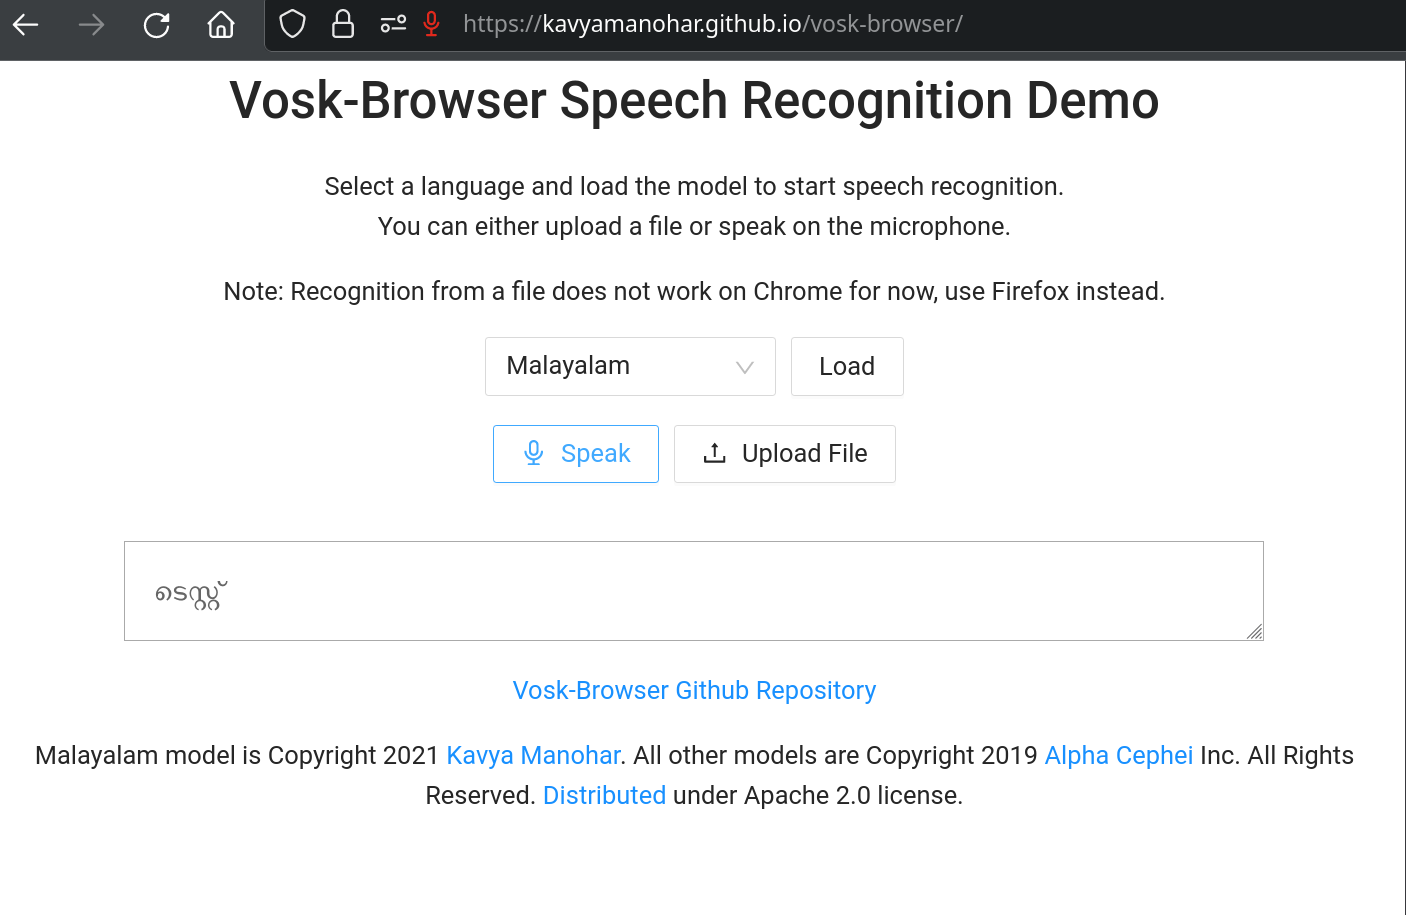
\includegraphics[width=0.8\linewidth]{Figures/chapter5-lvcsr/vosk.png}
	\caption{The Website demonstrating the ASR developed as per the description in this work}
	\label{fig:vosk}
\end{figure}
% \vspace{-0.5cm}
\section{Summary}

This chapter describes the development of an \gls{lvcsr} model for the Malayalam language. The development of an automated tool called Mlphon for \gls{g2p} conversion has made it possible to create a pronunciation lexicon for the language. The acoustic model was trained using \gls{lfmmi} discriminative training criteria with a \gls{tdnn}, which is the first attempt of its kind for Malayalam. The resulting \gls{lvcsr} model, when combined with the pronunciation lexicon built using Mlphon, achieved the best \gls{wer} on two different test datasets. However, the performance of the model was affected by the \gls{oov} rate, indicating the need for alternative language modelling techniques based on subword segmentation. The following chapter discusses these alternative language modelling techniques, which can potentially improve the performance of the \gls{lvcsr} model for Malayalam.